
\chapter{提案手法:セグメント化した IQ}
\label{sec:segment_IQ}
本論文では,IQ のタグ比較器の動作回数を削減するための手法として,IQ をセグメント化する手法を提案する.本章では,\refsec{segmented_IQ}で提案手法の基本アイデアに関して説明したあと,\refsec{second_tag_comp}で提案手法における第 2 ソース・タグ比較の削減方法である,\textbf{スワップ}と\textbf{サブ・セグメント}に関して説明する.最後に,\refsec{comp_estimate}で提案手法によるタグ比較回数削減の効果を概算する.

\section{IQ のセグメント化}
\label{sec:segmented_IQ}
本節では,提案手法の概要を説明した後,提案手法におけるウェイクアップとディスパッチに関して詳しく説明する.

\begin{figure}[htb]
  \centering
  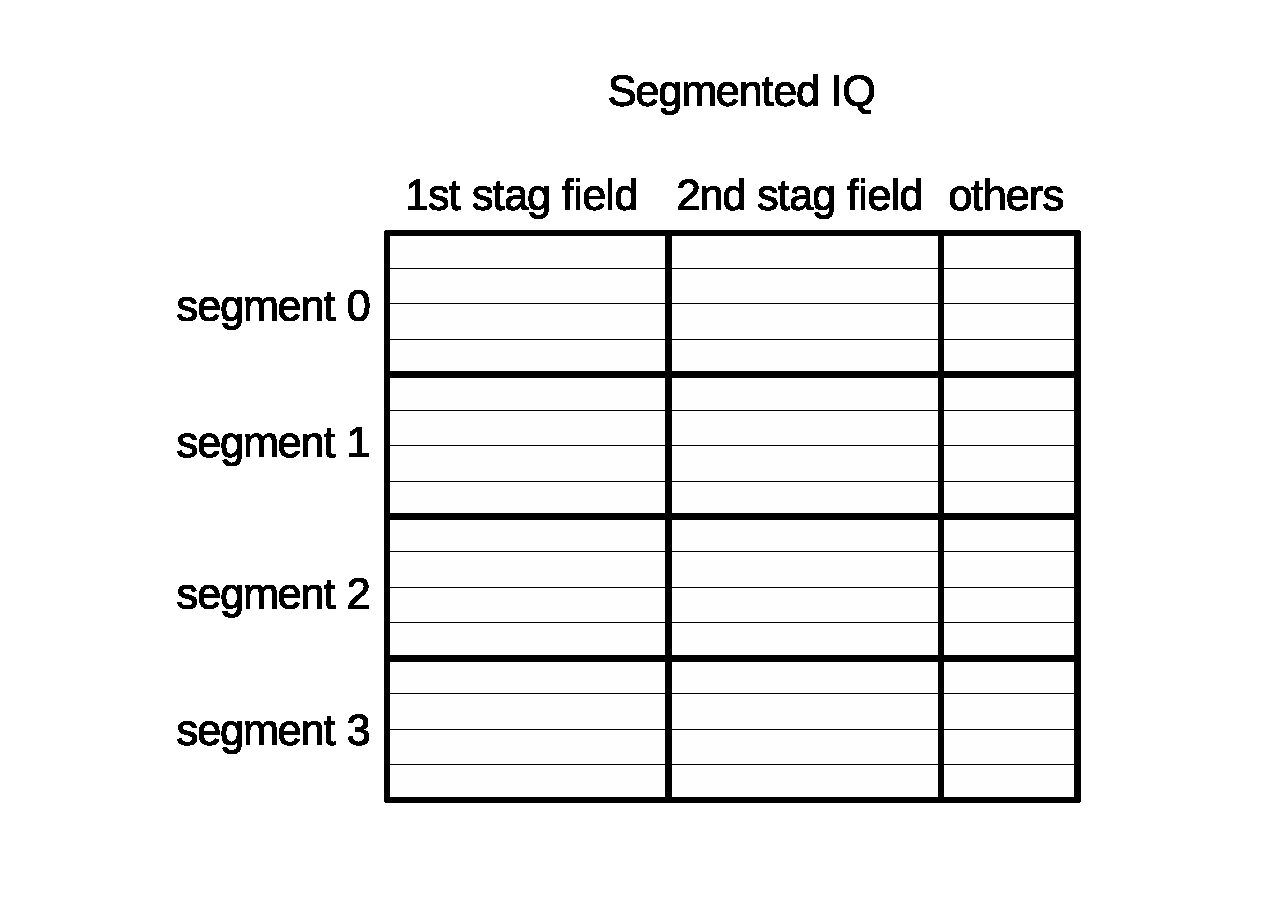
\includegraphics[keepaspectratio, scale=.8]{segmentedIQ}
  \caption{セグメント化した IQ}
  \label{fig:segmentedIQ}
\end{figure}

\subsection{提案手法の概要}
提案手法の基本アイデアは,大容量 CAM の電力削減に関する研究~\cite{Motomura1990paper, Motomura1990journal}から着想を得ている.この研究において提案されている手法では,CAM を複数の\textbf{セグメント}~\footnote{文献~\cite{Motomura1990paper, Motomura1990journal}ではバンクと呼ばれている.}に分割する.各セグメントには下位ビットが同一のデータのみを記録する.そして,タグ比較においては,比較対象のデータの下位ビットと,記録されているデータの下位ビットが一致するセグメントのみで比較を行う.これによって,比較器が動作する回数を「1/セグメント数」まで削減することができ,消費電力が削減できる.

本手法においても,\fig{segmentedIQ}に示すように IQ を複数のセグメントに分割する.各セグメントには,第 1 ソース・タグの下位ビットがセグメントの番号と一致する命令をディスパッチする.ウェイクアップ時の第 1 ソース・タグのタグ比較では,デスティネーション・タグの下位ビットとセグメントの番号が一致するセグメントのみでタグ比較を行う.これによって,第 1 ソース・タグのタグ比較回数を「1/セグメント数」に削減できる.

\subsection{提案手法におけるディスパッチ}
ディスパッチする IQ のエントリを決定する回路を\fig{dispatch}に示す.本手法では,フリー・リストをセグメントと同じ数だけ用意する.各フリー・リストは,対応するセグメントの空きエントリのインデクスを FIFO バッファで管理する.各フリー・リストからは IQ のインデクスが出力され,その中の1つを選択してディスパッチするエントリを決定する.どのフリー・リストからの出力を選択するかは,セグメント選択回路(図中の segment select logic)によって決定される.セグメント選択回路は,第 1 ソース・オペランドのタグ及びレディ・ビットと,各セグメントの空きエントリ数を入力とし,ディスパッチするセグメント番号を出力する.

セグメント選択回路の選択アルゴリズムについて説明する.セグメントの選択方法は,ディスパッチ時に第 1 ソース・オペランドがレディであるかによって異なるため,それぞれの場合に関して説明する.
\begin{itemize}
  \item \textbf{第 1 ソース・オペランドがレディでない場合}: 第 1 ソース・タグの下位ビットと番号が同じセグメントを選択する.選択されたセグメントに空きエントリがある場合,ディスパッチ可能であるため,対応するフリー・リストから読み出したエントリにディスパッチする.対応するセグメントに空きがない場合は,セグメントに空きが出るまでディスパッチをストールさせる.
  \item \textbf{第 1 ソース・オペランドがレディである場合}:この場合,第 1 ソース・タグの比較は行われないため,どのセグメントにディスパッチしても問題ない.このような場合を\textbf{セグメント・インディペンデント}と呼ぶ.この場合,空きエントリのあるセグメントから,ラウンドロビンでディスパッチするセグメントを選択しディスパッチする.
\end{itemize}
例として,第 1 ソース・オペランドがレディでなく,タグが 15(${\rm 1111_2}$)である命令を,\fig{segmentedIQ}に示す 4 つに分割された IQ にディスパッチする場合を考える.第 1 ソース・タグの下位 2 ビットが 3(${\rm 11_2}$)であるので,この命令は第 3 セグメントにディスパッチされる. 

なお,ソース・オペランドを使用しない命令も存在するが,そのような命令はディスパッチ時にソース・オペランドがレディであるものとして扱う.

\begin{figure}[htb]
  \centering
  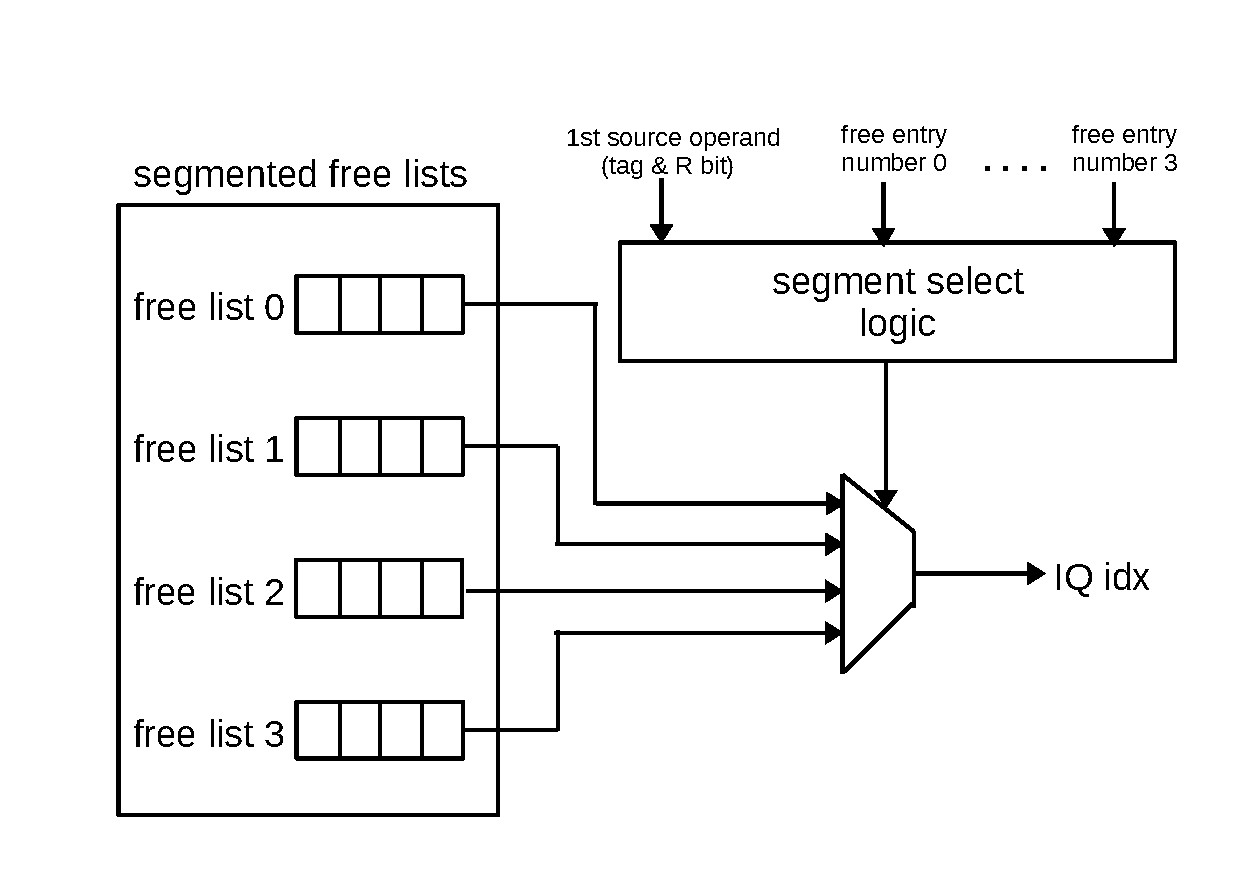
\includegraphics[keepaspectratio, scale=.8]{dispatch}
  \caption{提案手法におけるディスパッチエントリの決定回路}
  \label{fig:dispatch}
\end{figure}

\subsection{提案手法におけるウェイクアップ}
提案手法におけるウェイクアップでは,デスティネーション・タグの下位ビットがセグメント番号と一致するセグメントでのみ,第 1 ソース・タグのタグ比較器を動作させ比較を行う.一致しないセグメントはタグ比較器を動作させない.これは,デスティネーション・タグの下位ビットと番号が一致しないセグメントには,第 1 ソース・タグの下位ビットがデスティネーション・タグの下位ビットと異なる命令しか入っておらず,タグは必ず不一致となるためである.

例として,放送されたデスティネーション・タグが 6(${\rm 110_2}$)で,IQ が\fig{segmentedIQ}に示すように 4 つのセグメントに分割されている場合を考える.この場合,下位ビットは 2(${\rm 10_2}$)であるため,第 2 セグメントでのみ,第 1 ソース・タグのタグ比較を行う.

なお,第 2 ソース・タグのタグ比較に関しては,セグメントの番号とタグの下位ビットに関係性はないため,すべてのセグメントでタグ比較を行う必要がある.

提案手法におけるタグ比較の回路を\fig{segmentedIQ_wakeup}に示す.同図は 4 つのセグメントに分割された IQ のうち,第 0 セグメントのエントリにおける,第 1 ソース・タグの比較回路を示している.タグ・ビット数は 5 とし,発行幅を $IW$ とする.

タグ比較の動作を図中の番号を用いて説明する.\ctext{1}放送されるデスティネーション・タグの下位 2 ビットはデコーダ(SVSD:Segment-Validation Signal Decoder)へ送られる.SVSD はセグメント数だけ信号線を出力する.第 $n$ 番目の信号線は,第 $n$ セグメントでのタグ比較を有効化することを示す.つまり,デスティネーション・タグの下位ビットが $n$ の場合,$n$ 番目の出力線のみ $H$ を出力し,残りはすべて $L$ を出力する.SVSD の出力信号線のことを,以下, SVS(Segment-Validation Signal)と呼ぶ.

\ctext{2}AND ゲートによって,SVS が $H$ の場合にのみ,デスティネーション・タグの高位ビット及びその反転信号がタグ比較器へ入力される.\fig{segmentedIQ_wakeup}に示す回路は第 0 セグメントのタグ比較回路であるため,0 番目の SVS が AND ゲートに入力されている.

SVS が $H$ の場合,つまり,デスティネーション・タグの下位ビットとセグメント番号が一致していた場合のみ,比較器にデスティネーション・タグの高位ビットとその反転信号が送られ,ソース・タグの高位ビットと比較が行われる.SVS が $L$ の場合,デスティネーション・タグとその反転信号がどちらも $L$ としてタグ比較器へ入力される.この場合,デスティネーション・タグとその反転信号に接続されたプルダウン・トランジスタがすべて OFF となるため,マッチ線はディスチャージされず,電力を消費しない.

\ctext{3}タグ比較の結果,タグの高位ビットが一致した場合は,比較器から $H$ が出力される.

\ctext{4}タグ比較器が $H$ を出力し,かつ SVS が $H$ である場合に,タグ比較は一致となる.

\ctext{5}$IW$ 個の比較のいずれかが一致となった場合に,ソース・オペランドのレディ・ビットがセットされる.

SVSD の回路図を\fig{SVSD}に示す.SVSD はデスティネーション・タグの下位ビットのうち $\log_2(セグメント数)$ ビットの正転及び反転信号を入力とし,セグメント数分の SVS を出力するバイナリ・デコード回路である.SVSD は セグメント数分の AND ゲートで構成される.

図ではセグメント数が 4 の場合の SVSD を表記しており,デスティネーション・タグの下位 2 ビット($\log_2\:4$)を入力とし,SVS が 4 本出力される.赤字でタグの下位ビットが 2(${\rm 01_2}$)の場合を例示している.この場合,SVS2 のみ $H$ となり,その他の SVS は $L$ を出力する. 


\begin{figure}[thb]
  \centering
  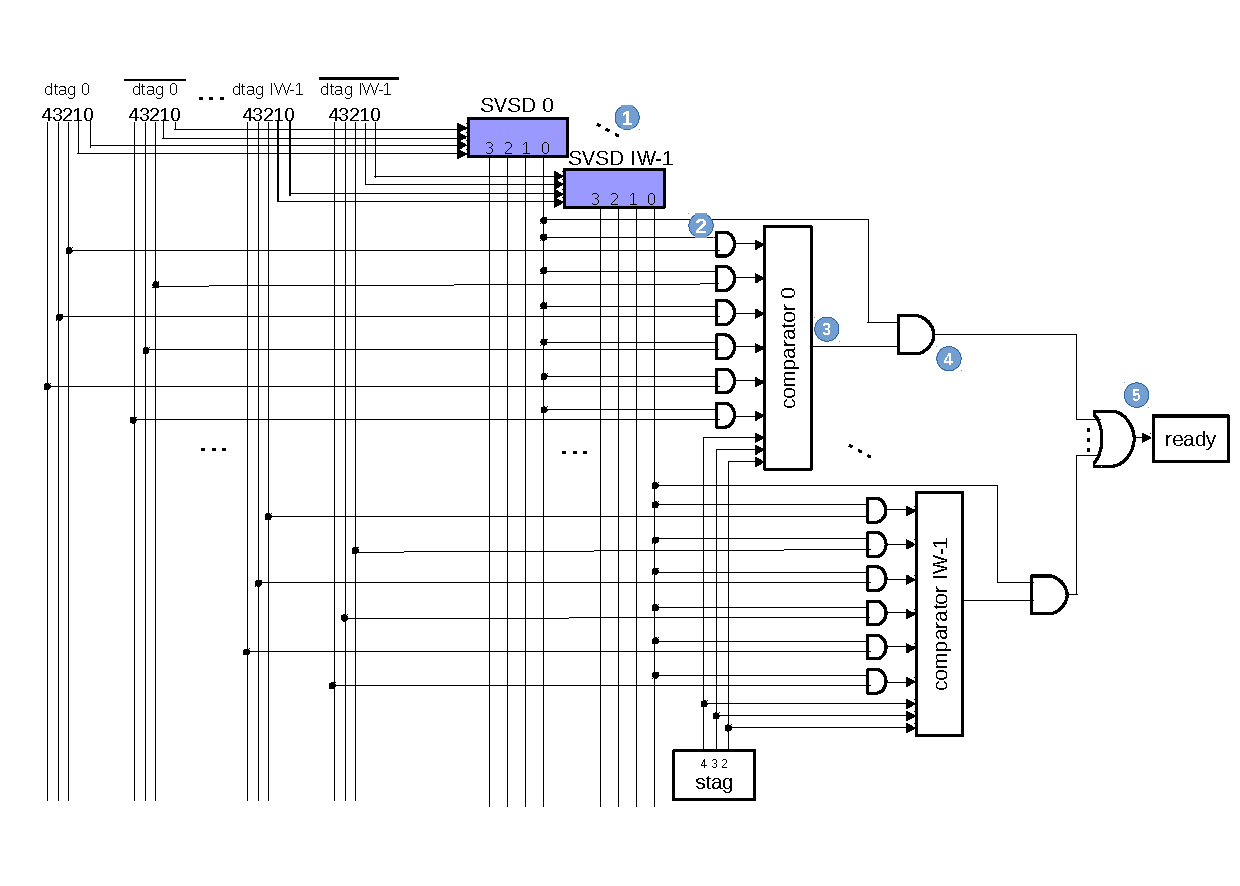
\includegraphics[keepaspectratio, scale=.8]{segmentedIQ_wakeup}
  \caption{提案手法におけるタグ比較回路(第 0 セグメント)}
  \label{fig:segmentedIQ_wakeup}
\end{figure}

\begin{figure}[htb]
  \centering
  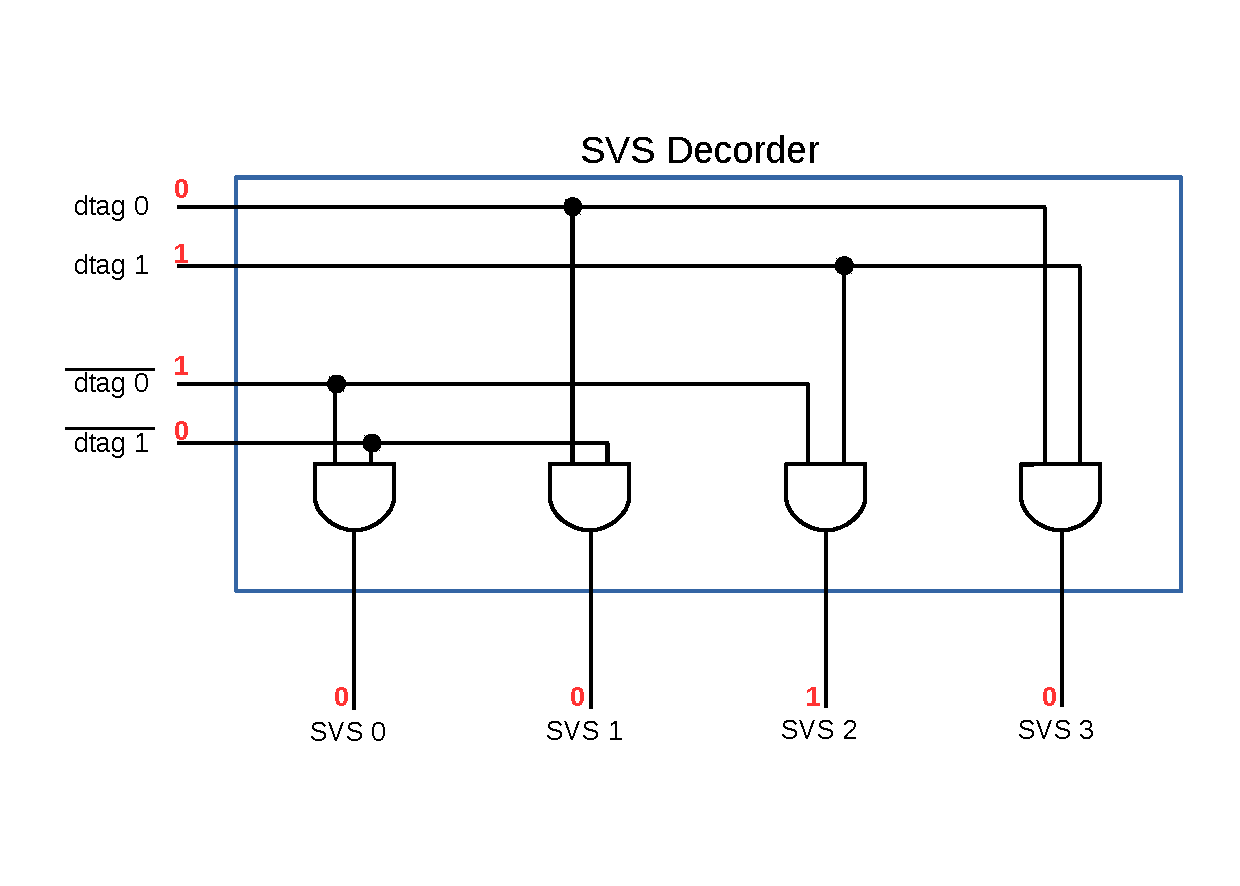
\includegraphics[keepaspectratio, scale=.8]{SVSD}
  \caption{SVSD(Segment-Validation Signal Decoder)}
  \label{fig:SVSD}
\end{figure}

% 図が後ろに行きすぎないように
\clearpage

%4 第 2 ソース・タグ比較の削減
\section{第 2 ソース・タグ比較の削減}
\label{sec:second_tag_comp}
\refsec{segmented_IQ}で述べた手法では,命令の第 2 ソース・タグのタグ比較回数は削減できない.そこで本節では,第 2 ソース・タグの比較回数の削減を可能とする\textbf{スワップ}と\textbf{サブ・セグメント}という 2 つの手法を提案する.

\subsection{スワップ}
\label{sec:swap}
スワップは,第 1 ソース・タグと第 2 ソース・タグを格納するフィールドを交換し,第 2 ソース・タグの下位ビットをもとにディスパッチするセグメントを決定する手法である.以下で詳しく説明する.

第 1 ソース・オペランドがレディで,第 2 ソース・オペランドがレディでない場合について説明する.この場合,\refsec{segmented_IQ}で説明した方法では,命令はセグメント・インディペンデントとしてディスパッチされる.第 1 ソース・オペランドは既にレディであるため,比較は第 2 ソース・タグについてのみ行われるが,第 2  ソース・タグのタグ比較は全てのセグメントで行われるため,タグ比較の回数は削減されない.

そこでこのような場合に,第 1 ソース・タグと第 2 ソース・タグを交換し(スワップ),第 2 ソース・タグの下位ビットを使用してディスパッチするセグメントを選択する.これにより,\refsec{segmented_IQ}で述べたセグメント化の効果でタグ比較回数が削減される.なお,スワップではタグを交換するが,ペイロード RAM に格納するソース・タグ(物理レジスタ番号)を交換するわけではないので,命令の意味は保持される.

\subsubsection{スワップを行う場合のセグメント選択アルゴリズム}
セグメント選択回路は,\tab{agg_algorithm}に示すアルゴリズムによってディスパッチするセグメントを決定する.なお,表中のソース・タグの状態とは,ディスパッチ時にソース・オペランドがレディであるかどうかを示しており,(第 1 ソース・オペランド,第 2 ソース・オペランド)の形式で,R がレディであることを,NR がレディでないことを表す.

\begin{table}[htb]
  \caption{スワップを行う場合のセグメント選択アルゴリズム}
  \footnotesize
  \center
   \begin{tabular}{|l|l|} \hline \hline
    ソース・タグの状態 & アルゴリズム \\ \hline
    (NR,NR) & 第 1 ソース・タグでセグメントを選択する. \\ \hline
    (R,NR) & スワップを行い,第 2 ソース・タグでセグメントを選択する.\\ \hline
    (NR,R) & 第 1 ソース・タグでセグメントを選択する.\\ \hline
    (R,R) & セグメント・インディペンデントとしてラウンドロビンでセグメントを選択する. \\ \hline
  \end{tabular}
  \label{tab:agg_algorithm}
\end{table}
なお,両ソース・オペランドがレディのとき以外で,選択されたセグメントに空きがない場合は,ディスパッチをストールして当該のセグメントに空きが出るまで待ち合わせる.

\subsection{サブ・セグメント}
\label{sec:sub_segment}
サブ・セグメント方式は,第 1 ソース・タグの下位ビットに応じて分割されるセグメントを,第 2 ソース・タグの下位ビットに応じてさらに細かく分割する方式である.第 2 ソース・タグの下位ビットによる分割をサブ・セグメント(S-seg)と呼び,従来の第 1 ソース・タグによる分割をサブ・セグメントに対応してメイン・セグメント(M-seg)と呼ぶこととする.

サブ・セグメントを導入した IQ の分割を\fig{sub_segment}に示す.黒色の枠で示す各メイン・セグメントを,赤色と青色で示すようにさらにサブ・セグメントに分割する.同図は,メイン・セグメント数が 4 ,サブ・セグメント数が 2 の場合の例を表しており, IQ は合計 $4 \times 2 = 8$ 個のセグメントに分割される.各セグメントの左には,(M-seg,S-seg)という形式でメイン及びサブ・セグメントの番号を表している.

サブ・セグメント方式について,ディスパッチとウェイクアップの動作をそれぞれ説明する.

\begin{figure}[htb]
  \centering
  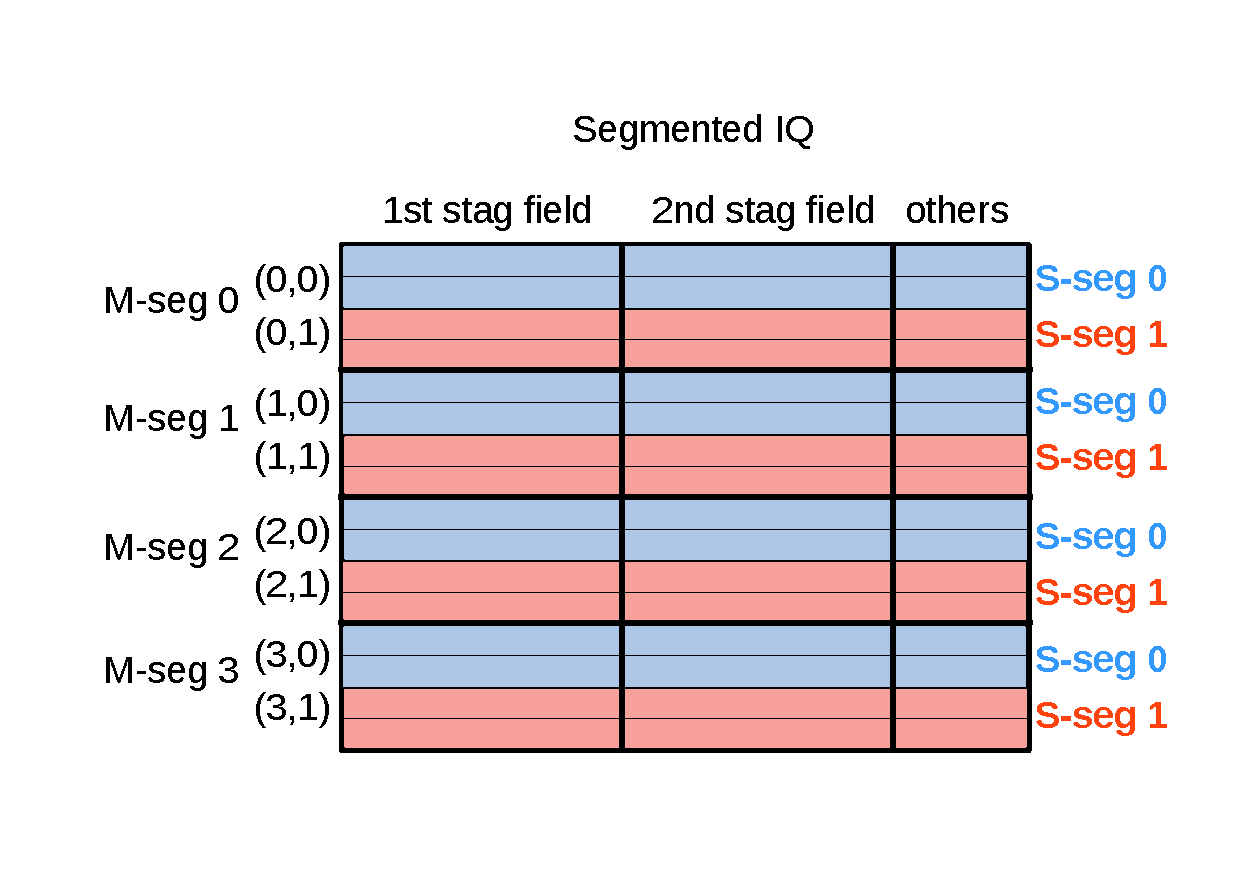
\includegraphics[keepaspectratio, scale=.8]{sub_segment}
  \caption{サブ・セグメントを実装した IQ}
  \label{fig:sub_segment}
\end{figure}

\subsubsection{サブ・セグメントにおけるディスパッチ}
サブ・セグメント方式におけるディスパッチにおいては,フリー・リストを M-seg $\times$ S-seg だけ用意する.\fig{sub_segment}に示した例の場合 8 個のフリー・リストが必要となる.

サブ・セグメント方式におけるセグメント選択のアルゴリズムに関して説明する.アルゴリズムはソース・オペランドのレディ状況によって異なるため,以下ですべての場合に関して説明する.説明を簡単にするため,命令 $p5 = p13 + p6$ を,\fig{sub_segment}に示す IQ にディスパッチする場合について例示する.第 1 ソース・タグが 13 で,第 2 ソース・タグが 6 である.
\begin{itemize}
  \item \textbf{両ソース・オペランドともレディでない場合}:第 1 ソース・タグでメイン・セグメントを,第 2 ソース・タグでサブ・セグメントを選択する.例の場合,第 1 ソース・タグ 13(${\rm 1101_2}$) の下位ビット 1(${\rm 01_2}$)より,メイン・セグメントは 1 となる.また,第 2 ソース・タグ 6(${\rm 110_2}$) の下位ビット 0(${\rm 0_2}$)より,サブ・セグメントは 0 となる.従って(1,0)のセグメントを選択する. 
  \item \textbf{第 1 ソース・オペランドのみレディである場合}:第 2 ソース・タグでサブ・セグメントを選択する.例の場合,第 2 ソース・タグ 6(${\rm 110_2}$) の下位ビット 0(${\rm 0_2}$)より,サブ・セグメントは 0 となる.第 1 ソース・オペランドは既にレディであるため,メイン・セグメントの制限はない.従って,(0,0),(1,0),(2,0),(3,0)のいずれかのセグメントをラウンドロビンで選択する.このように,メイン・セグメントの制限がない場合をメイン・セグメント・インディペンデント(M-seg インディペンデント)と呼ぶこととする.
  \item \textbf{第 2 ソース・オペランドのみレディである場合}:第 1 ソース・タグでメイン・セグメントを選択する.例の場合,第 1 ソース・タグ 13(${\rm 1101_2}$) の下位ビット 1(${\rm 01_2}$)より,メイン・セグメントは 1 となる.第 2 ソース・オペランドは既にレディであるため,サブ・セグメントの制限はない.従って,(1,0)または(1,1)のいずれかのセグメントをラウンドロビンで選択する.このように,サブ・セグメントの制限がない場合をサブ・セグメント・インディペンデント(S-seg インディペンデント)と呼ぶこととする.
  \item \textbf{両ソース・オペランドがレディである場合}:M-seg インディペンデントかつ S-seg インディペンデントであるため,空きのあるすべてのセグメントからラウンドロビンで選択する.
\end{itemize}

\subsubsection{サブ・セグメントにおけるウェイクアップ}
第 1 ソース・タグの比較は,デスティネーション・タグの下位ビットがメイン・セグメント番号と一致するセグメントのみで行う.また,第 2 ソース・タグの比較は,デスティネーション・タグの下位ビットがサブ・セグメント番号と一致するセグメントのみで行う.このような比較により,第 1 ソース・タグだけでなく,第 2  ソース・タグの比較に関しても,「1/サブ・セグメント数」まで削減が可能となる.

\subsubsection{サブ・セグメントとスワップの併用}
サブ・セグメント方式はスワップと併用することが可能である.併用する場合は,ディスパッチ時に第 1 ソース・オペランドのみレディである場合の選択アルゴリズムを,以下のように変更する.
\begin{quote}
  \textbf{第 1 ソース・オペランドのみレディである場合}:スワップを行い,第 2 ソース・タグでメイン・セグメントを選択する.例の場合,第 2 ソース・タグ 6(${\rm 110_2}$) の下位ビット 2(${\rm 10_2}$)より,メイン・セグメントは 2 となる.第 1 ソース・オペランドは既にレディであるため,S-seg インディペンデントである.従って,(2,0)または(2,1)のいずれかのセグメントを選択する.
\end{quote}
サブ・セグメント方式とスワップを併用することによって,ディスパッチ時に第 1 ソース・オペランドのみレディである命令におけるタグ比較回数の削減が「1/サブ・セグメント数」から「1/メイン・セグメント数」となる.従って,\fig{sub_segment}に示した分割のようにメイン・セグメント数がサブ・セグメント数よりも多い場合に,タグ比較回数をより多く削減できる.

サブ・セグメントとスワップを併用する場合のセグメントの選択アルゴリズムを\tab{agg_algorithm_subseg}にまとめる.

\begin{table}[htb]
  \caption{スワップを行う場合のセグメント選択アルゴリズム(サブ・セグメント併用)}
  \footnotesize
  \center
   \begin{tabular}{|c|p{13cm}|} \hline \hline
    ソース・タグの状態 & アルゴリズム \\ \hline
    (NR,NR) & 第 1 ソース・タグでメイン・セグメントを,第 2 ソース・タグでサブ・セグメントを選択. \\ \hline
    (R,NR) & スワップを行い,第 2 ソース・タグでメイン・セグメントを選択する.サブ・セグメントは S-seg インディペンデントとしてセグメントを選択.\\ \hline
    (NR,R) & 第 1 ソース・タグでメイン・セグメントを選択する.サブ・セグメントは S-seg インディペンデントとしてセグメントを選択.\\ \hline
    (R,R) & M-seg インディペンデントかつ S-seg インディペンデントとしてセグメントを選択. \\ \hline
  \end{tabular}
  \label{tab:agg_algorithm_subseg}
\end{table}

\section{提案手法におけるタグ比較回数の概算}
\label{sec:comp_estimate}
提案手法におけるタグ比較回数削減の効果を概算する.なお,サブ・セグメントを使用する場合も使用しない場合も,(R,NR)の場合にスワップを行うものとする.

概算するにあたり,次の 2 つの仮定をおく.
\begin{enumerate}
  \item 命令のソース・タグは 50\% の確率でディスパッチ時にレディであるとする.つまり,(NR,NR),(R,NR),(NR,R),(R,R) である命令の数は全て等しいとする.
  \item 提案手法による IQ の容量効率の低下(詳しくは\refsec{switch}で説明する)は全く生じないとする.
\end{enumerate}
上記の仮定をおいた場合に,提案手法を使用した場合のタグ比較回数は,以下の式で計算することができる(式の導出は\refapp{appendix1}で示す).

\[
  \frac{3}{4}\times\frac{1}{M\_seg} + \frac{1}{4}\times\frac{1}{S\_seg}
\]
ここで,$M\_seg$ はメイン・セグメント数を, $S\_seg$ はサブ・セグメント数を表す.なお,サブ・セグメントを使用しない場合は,$M\_seg$ をセグメント数とし,$S\_seg = 1 $ として計算すれば良い.

この式を用いて,本論文にて評価を行った全てのセグメント数の組み合わせにおける,タグ比較回数の概算を行った.その結果を\tab{comp_estimate}に示す.表に示しているタグ比較回数は,セグメント化しない通常の IQ に対する相対タグ比較回数である.

なお,以降の説明において,(メイン・セグメント数,サブ・セグメント数) の形式でセグメント数を表記する.また,サブ・セグメントを使用しない場合は,サブ・セグメント数は 1 と表記する.例えば,サブ・セグメントを使用せず,セグメント数を 16 とする場合は(16,1)と表記し,サブ・セグメントを使用し,メイン・セグメント数を 8 ,サブ・セグメント数を 2 とする場合(8,2)と表記する.

\begin{table}[htb]
  \caption{タグ比較回数の概算}
  \footnotesize
  \center
    \begin{tabular}{c|c|c} \hline \hline
    総セグメント数 & (M-seg,S-seg) & 相対タグ比較回数(\%) \\ \hline
    4 &(4,1) & 44 \\
    &(2,2) & 50 \\ \hline
    8 &(8,1) & 34 \\
    &(4,2) & 31 \\ \hline
    &(16,1) & 30 \\
    16 &(8,2) & 22 \\
    &(4,4) & 25 \\ \hline
    &(32,1) & 27 \\
    32 &(16,2) & 17 \\
    &(8,4) & 16 \\ \hline
  \end{tabular}
  \label{tab:comp_estimate}
\end{table}

表より,総セグメント数が多くなるほど,タグ比較回数が少なくなることがわかる.また,総セグメント数が同じ場合,総セグメント数が 4 の場合を除いて,サブ・セグメントを使用する方がタグ比較回数が少ないことがわかる.これは,サブ・セグメントを用いることによって,(NR,NR)の場合に第 2 ソース・タグの比較回数が削減できるようになる効果が大きいためである.

なお,実際のタグ比較回数は,\refsec{switch}で説明する IQ の容量効率の低下により,計算した概算値よりも少なくなる.